\documentclass{article}
\usepackage{tikz,amsmath,siunitx}
\usepackage{pgfplots}
\usepackage{listings}
\usetikzlibrary{arrows,snakes,backgrounds,patterns,matrix,shapes,fit,calc,shadows,plotmarks}
%\usepackage[graphics,tightpage,active]{preview}
%\PreviewEnvironment{tikzpicture}
%\PreviewEnvironment{equation}
%\PreviewEnvironment{equation*}
\title{CS540 Practice Assignment 7}
\author{Dustin Ingram, Aaron Rosenfeld, Tom Wambold}
\newlength{\imagewidth}
\newlength{\imagescale}
\pagestyle{empty}
\thispagestyle{empty}
\lstset{breaklines=true}
\begin{document}
\maketitle
\newpage
\section{Tasks}
\begin{enumerate}
    \item Implement and time a vector version of W\_4 using sse2.
    \item Implement and time a vector version of W\_8 using sse.
    \item Implement and time a vector version of the recursive WHT algorithm.
\end{enumerate}
\section{Results}
\subsection{Timings for vectorized W\_4, W\_8 and Recursive}
  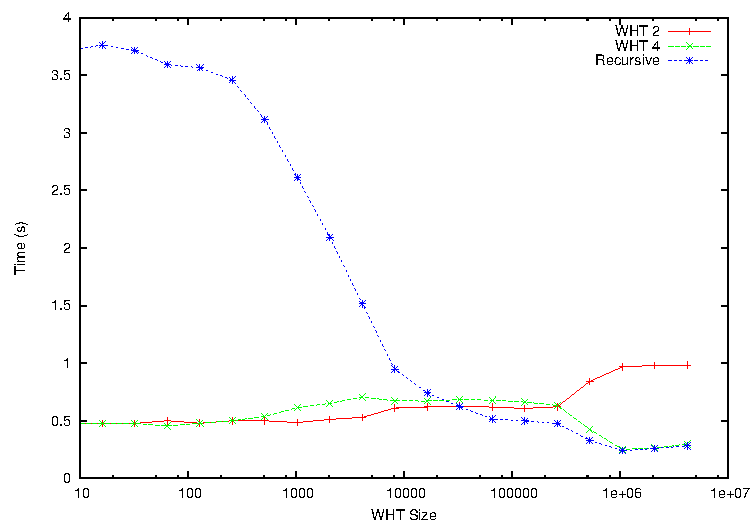
\includegraphics[width=\textwidth]{p7.pdf}
\end{document}

